% !TEX root = ../ClassicThesis_DEIB.tex

\chapter{Experimental results} \label{chap:experimentalResults}

On the field sessions were a crucial point in the validation of \ac{GRAPE} system, for two main reasons:
\begin{enumerate}
	
	\item Robotics is a field that, by definition, requires interaction with the physical world: both the components of the robot itself, and the environment. Thus, simulation could strongly speed up the the development in certain phases, but the creation of a robotic system cannot opt out of experimental sessions. This consideration is especially true in agricultural robotics field, because a simulated environment or a laboratory environment are extremely likely to be too different from the actual robot environment to be significant, \textit{e.g.} in terms of light conditions, terrain structure, sensor noise.

	\item As explained in Section \ref{sec:grapeProjectDescription}, the research team included members from both Politecnico di Milano and Eurecat, that are located in two different countries. Even if this should not have been a big problem, the division of labor created significant inefficiencies because:
	\begin{itemize}
		\item even if the sensor fusion and navigation parts were assigned to Politecnico, the Husky unmanned ground vehicle was property of Eurecat, so it was in Barcellona.
		\item even if the analysis of the vine scan in order to detect the most suitable deployment point was in charge of Eurecat, the arm was property of Politecnico so it was in Milano.
	\end{itemize}
	This problem was mitigated by the logging tool of \ac{ROS} (\textit{rosbag} package we mentioned in Section \ref{sec:robotOperatingSystem}), that demonstrated its potential in such a situation: \textit{bags} recorded during (non-autonomous) navigation sessions of the Husky were very useful to test the sensor fusion system, while \textit{bags} of the laser scans sensed during execution of the scan motion in front of the mockup vine (owned by Politecnico team, see Figure \ref{fig:mockupPlant}), were used by Eurecat team to test the point cloud creation and analysis. 
\par However, the usage of \textit{bags} in our context showed two main weaknesses, the first of which is specific of our context, while the second is intrinsic to the use of recorded data:
\begin{itemize}
	\item autonomous navigation algorithms cannot be tested by means of recorded data \textit{bags} because, during an autonomous navigation session, the data that are sensed while using a specific navigation algorithm depend on the choices of the algorithm itself; the same reasoning does not apply to neither sensor fusion nor point cloud analysis tasks.
	For this reason, the only way to test a navigation algorithm except for \textit{on-the-field} experiments is via simulation by means of a physical simulator. Some effort were spent in this direction before the beginning of this thesis work (see Section \ref{sec:thesisInGrape}), but very few \textit{on-the-field} tests have been enough to show that the simulated environment was way too different from the real one for the test to be significant.
	\item validation of algorithms by means of recorded data significantly increases the risk of overfitting, \textit{i.e.}, adapting the model to perform properly only on the data in the (few) \textit{bags} at disposal, and not on new data coming, for example, from an \textit{on-the-field} experiment. The best ways to decrease the probability of overfitting are:
	\begin{itemize}
		\item use as many bags as possible to test the algorithms during development.
		\item test the system in the real environment as often as you can. Remember, however, that sometimes overfitting can occur also in real environment, in less obvious way. For example, the ROAMFREE configuration executed in Garriguella during the first integration week was absolutely ineffective when applied in Casciana Terme vineyard, because it fitted too tightly the features of Garriguella vineyard thus it didn't represent a general solution.
	\end{itemize}
\end{itemize}

\end{enumerate}

\section{Sensor fusion}\label{sec:resultsOdometry}

Since the final sensor fusion system included data from GPS, we can exploit satellite imagery to better visualize and evaluate the sensor fusion output. For this purpose, we used the \textit{Rviz\_satellite} plugin for Rviz. In this section we'll show data recorded during a 13 minutes long autonomous navigation session of the Husky, executed across three different rows in the Garriguella vineyard, during the third integration week, in March 2018. In our case, satellite images also provide a very coarse-grained ground truth about the path, because we know the rows that the robot has actually traversed during navigation.

\par As explained in Section \ref{sec:odometrySystem}, we expected a very untrustworthy wheels odometry, and the experimental results actually proved it. In Figure \ref{fig:wheelsOdometryRes} you can see the pose estimated by the raw wheels velocities only. It's easy to notice that there's no way to use it as unique odometry source: the wheels slippage, especially during rotational movements, makes the estimated path completely different from the actual one. The data from GPS, shown in Figure \ref{fig:gpsRawRes}, are instead really accurate, since RTK correction was used. 
\par Indeed, the final estimated odometry, that you can see in Figure \ref{fig:robLocResult}, is very close to the the plotted GPS data in Figure \ref{fig:gpsRawRes}. However, a sensor fusion based on GPS only would not be a real solution, because:
\begin{itemize}
	\item the GPS update frequency is low (\textasciitilde1 Hz), so other sensors are required to improve the estimate between two GPS measures
	\item the GPS does not provide information about the orientation
	\item GPS availability, especially with RTK correction, is not guaranteed all over the world, so other sensors must be available to compensate if required
\end{itemize}

\begin{figure}
	\centering
	\subfloat[]{%
		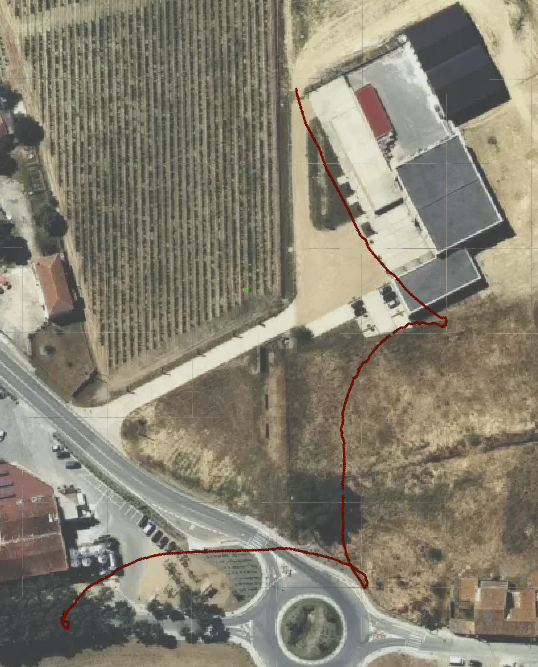
\includegraphics[width=0.65\textwidth]{Images/experimental_data/wheels_3.png}
		\label{fig:wheelsOdometryRes}} \\
	\subfloat[]{%
		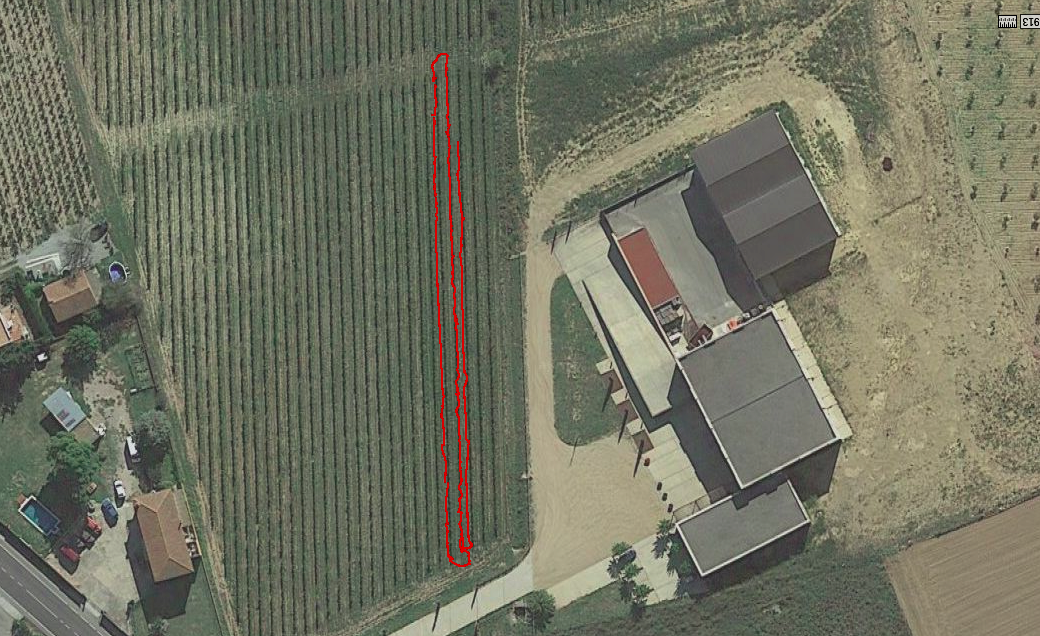
\includegraphics[width=0.7\textwidth]{Images/experimental_data/gpsRaw_dark.png}
		\label{fig:gpsRawRes}}
	\caption{\textit{Pose estimation in time using raw wheels odometry (Figure \ref{fig:wheelsOdometryRes}), and using GPS (Figure \ref{fig:gpsRawRes}).}}
	\label{fig:sensorFusionInputs}
\end{figure}

\begin{figure}
	\centering
	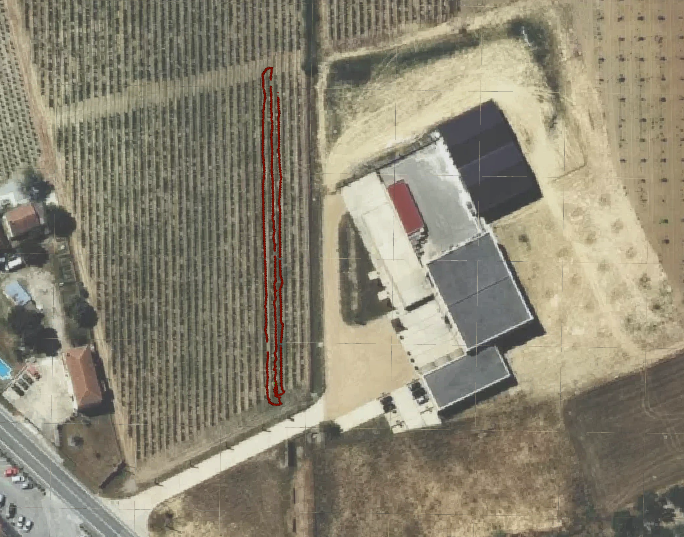
\includegraphics[width=0.75\textwidth]{Images/experimental_data/rob_loc_result.png}
	\caption{\textit{The odometry estimated by Robot Localization sensor fusion framework, fusing (among others) the pose estimated by the wheels (see Figure \ref{fig:wheelsOdometryRes}) and by the GPS (see Figure \ref{fig:gpsRawRes})}}
	\label{fig:robLocResult}
\end{figure}

\section{Navigation}

In the odometry system, the satellite imagery provided, as already stated, a sort of coarse-grained ground truth. The same reasoning cannot be applied to navigation operations, thus the evaluation of a navigation system by means of a quantitative metric is not easy.
	\par Because of the tight deadlines in the \ac{GRAPE} project, no particular effort was put in this topic, so we limited ourselves to observe high-level qualitative features of the local planner behavior (\textit{e.g} number of times the robot got stuck in obstacles during navigation, smoothness of the movement) to assess both the inadequacy of \textit{Dynamic Window Approach} planner, and the proper functionality \textit{Timed Elastic Band} planner.
	\par In Figure \ref{fig:result_navigation} you can see a frame of the same autonomous navigation session in Garriguella mentioned in Section \ref{sec:resultsOdometry}. The global navigation plan that the robot is following is drawn as a green line, while the shorter red line represents the local plan computed by  \textit{Timed Elastic Band}. The ability of this algorithm to deal with winding paths is clear in this image.

\par In Figure \ref{fig:mappingResults}, you can see the result of mapping process executed with Gmapping as \ac{SLAM} algorithm and Robot Localization as sensor fusion system. In both of them the vineyard structure is clearly visible.


\begin{figure}
	\begin{minipage}[c]{.5\textwidth}
	\centering
	\subfloat[]{%
		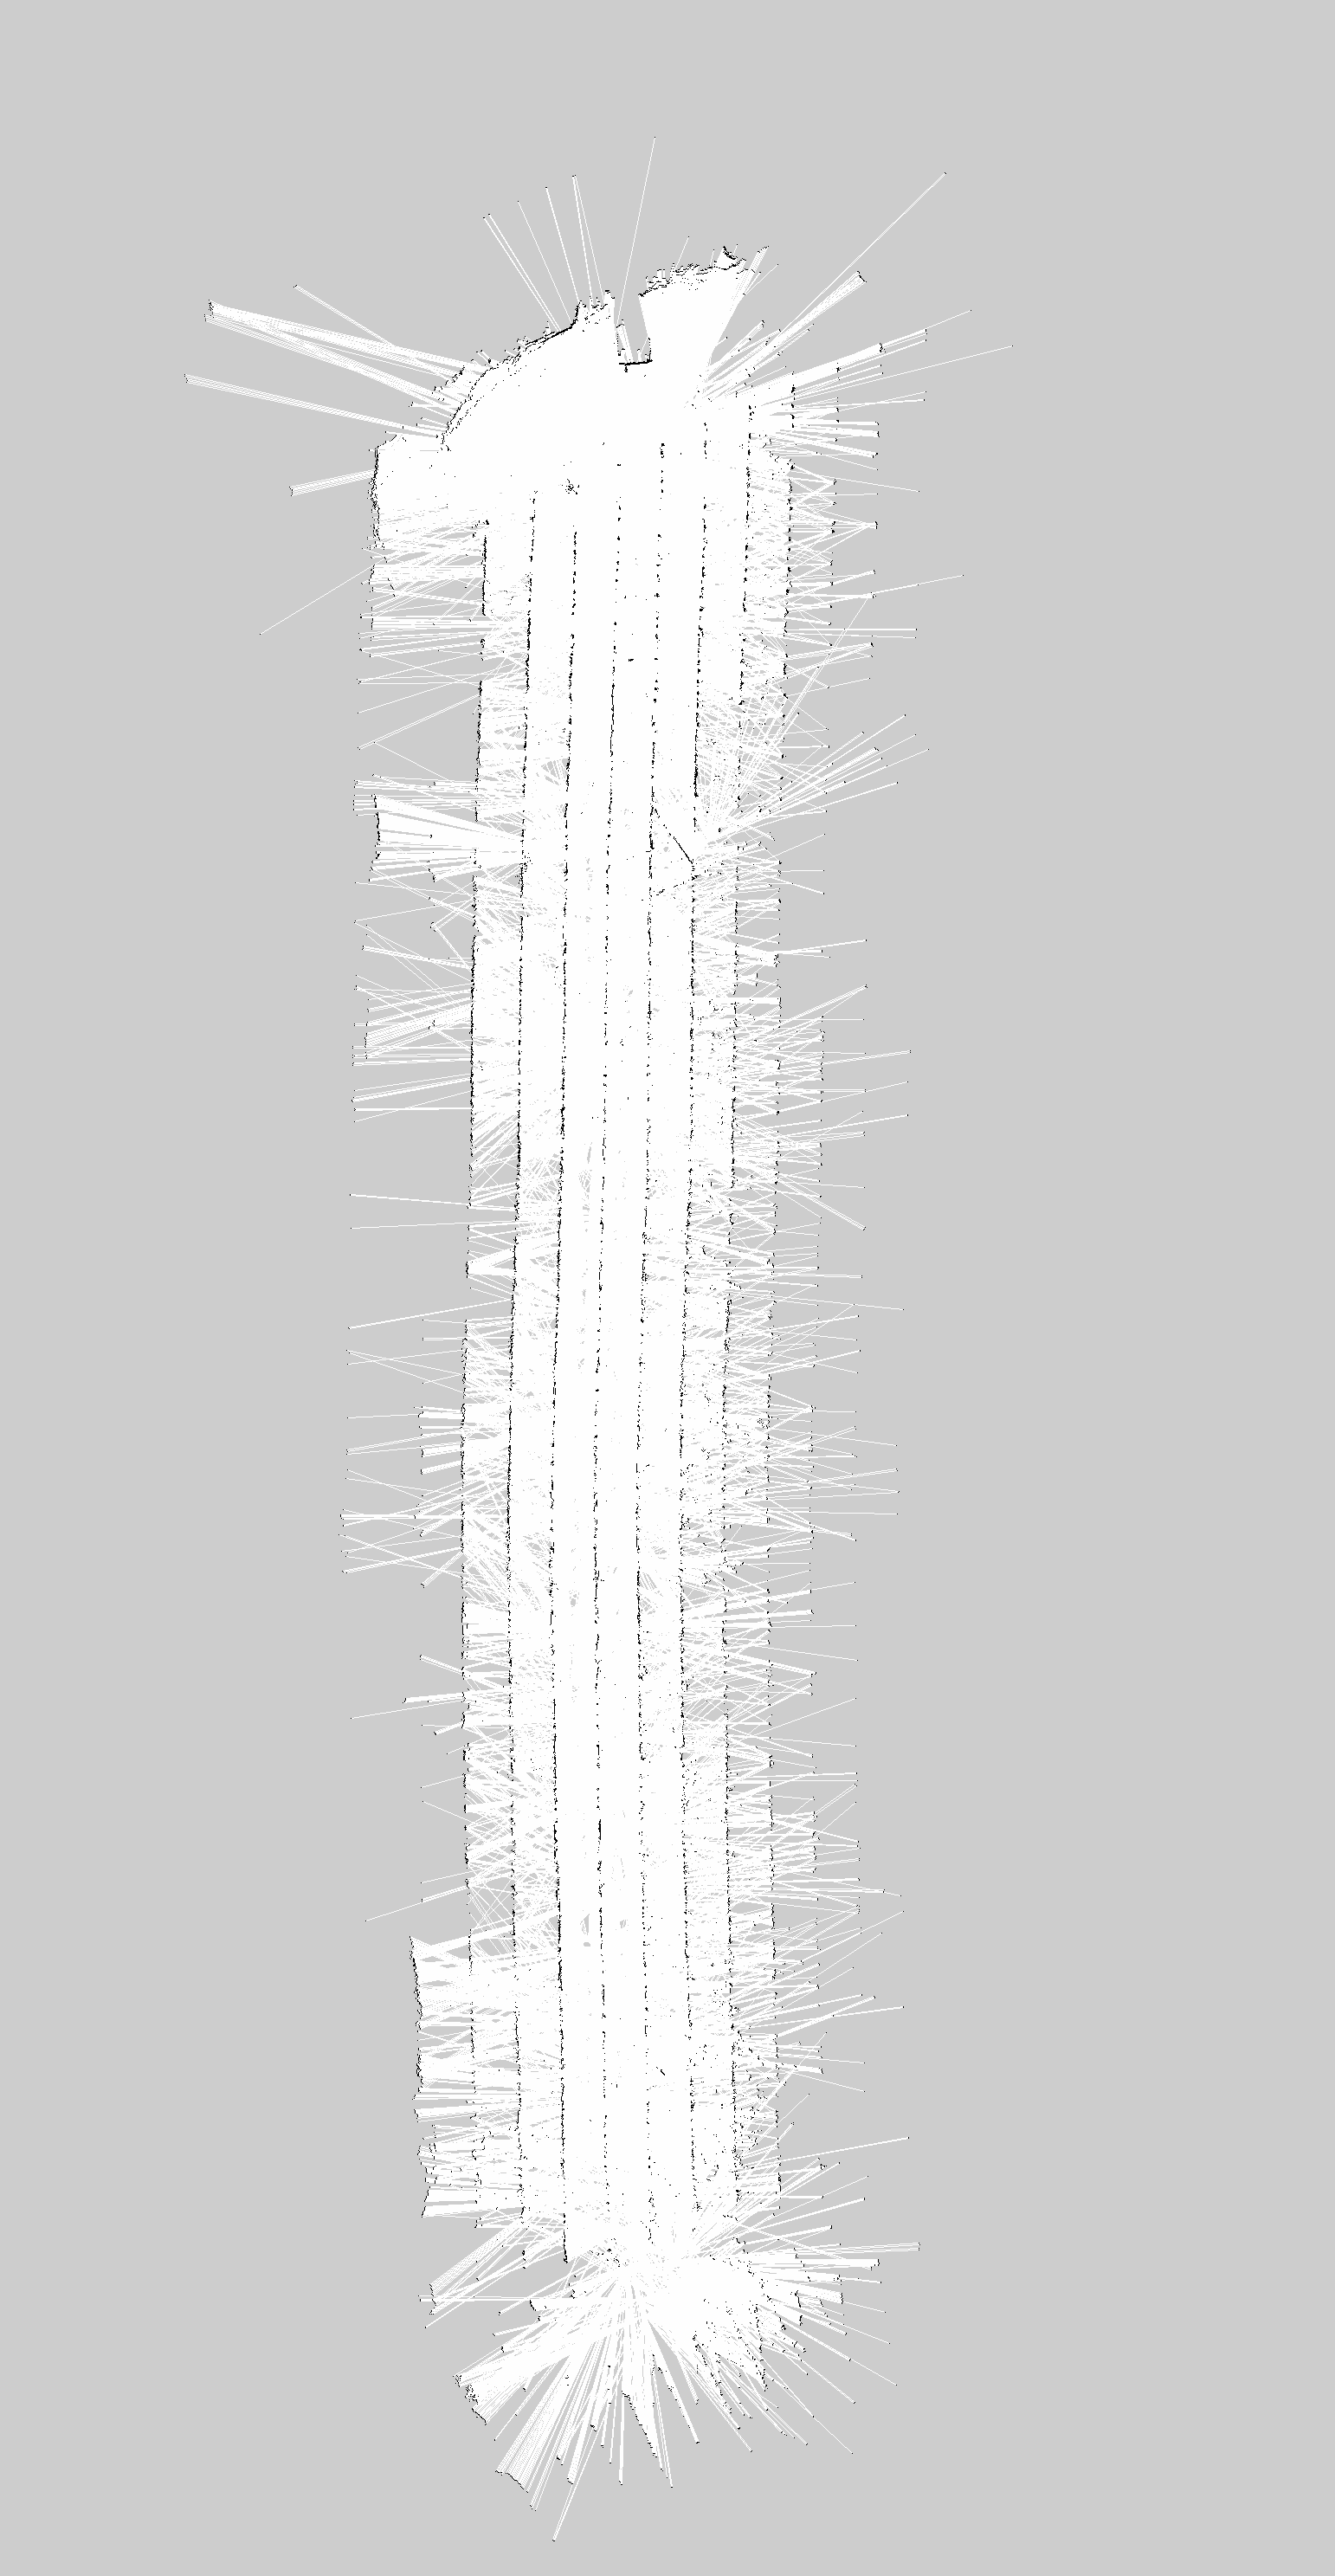
\includegraphics[width=0.7\textwidth]{Images/experimental_data/masLlunes_map.png}
		\label{fig:mapResult_masLlunes}}
	\end{minipage}
	\begin{minipage}[c]{.5\textwidth}
	\subfloat[]{%
		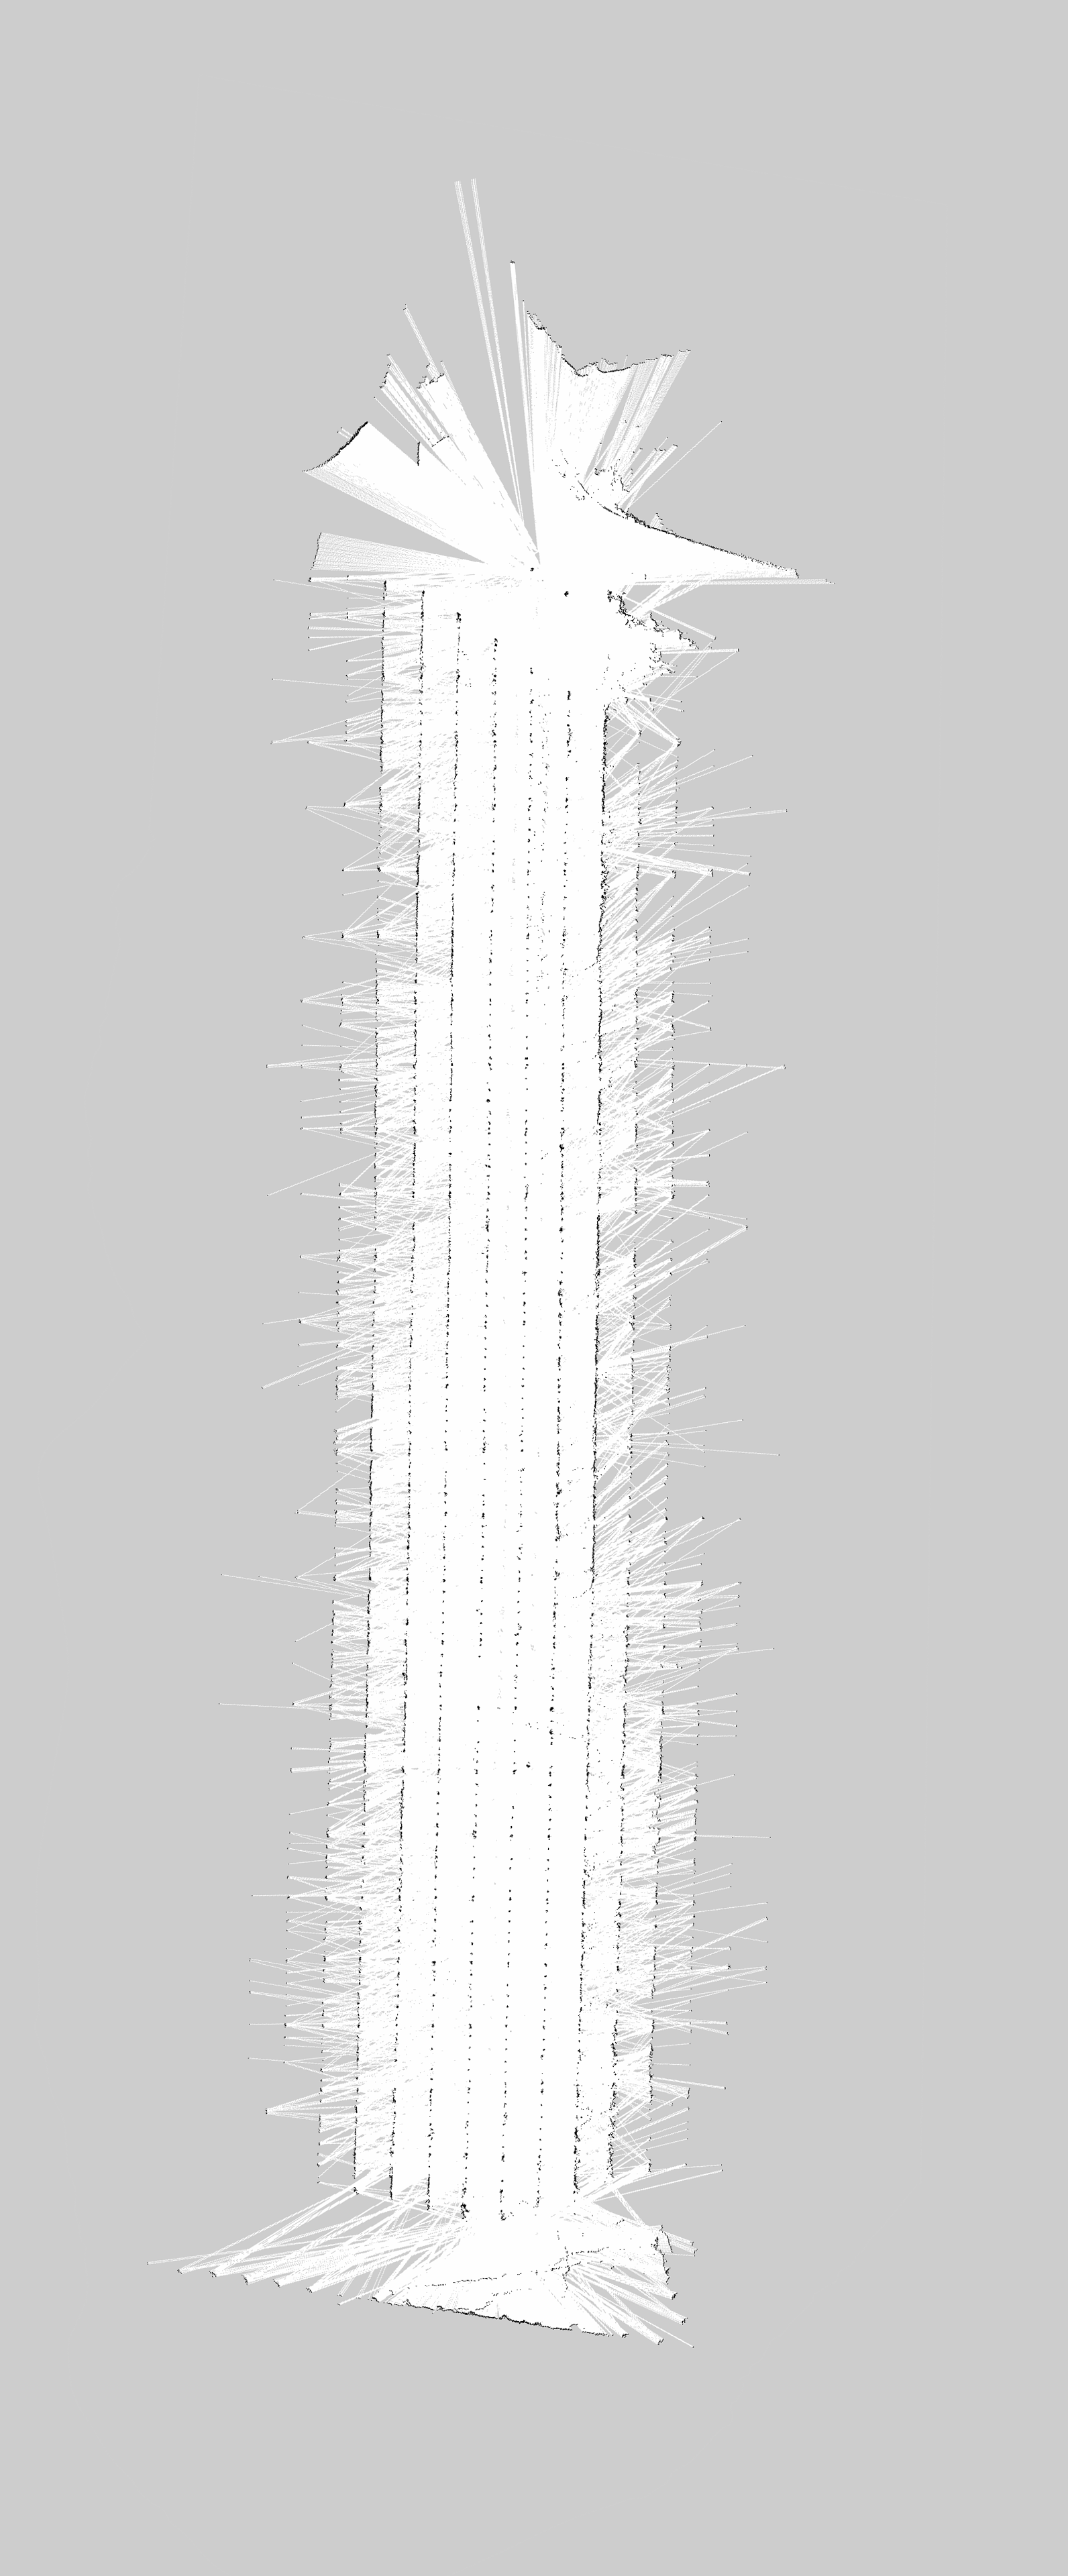
\includegraphics[width=0.65\textwidth]{Images/experimental_data/toscana_map.png}
		\label{fig:mapResult_toscana}}
	\end{minipage}
	\caption{\textit{Output of mapping phase, using Gmapping as \ac{SLAM} algorithm and Robot Localization as sensor fusion framework. The map of Garriguella vineyard in Figure \ref{fig:mapResult_masLlunes}, the Casciana Terme one in Figure \ref{fig:mapResult_toscana}.}}
	\label{fig:mappingResults}
\end{figure}


\begin{figure}
	\centering
	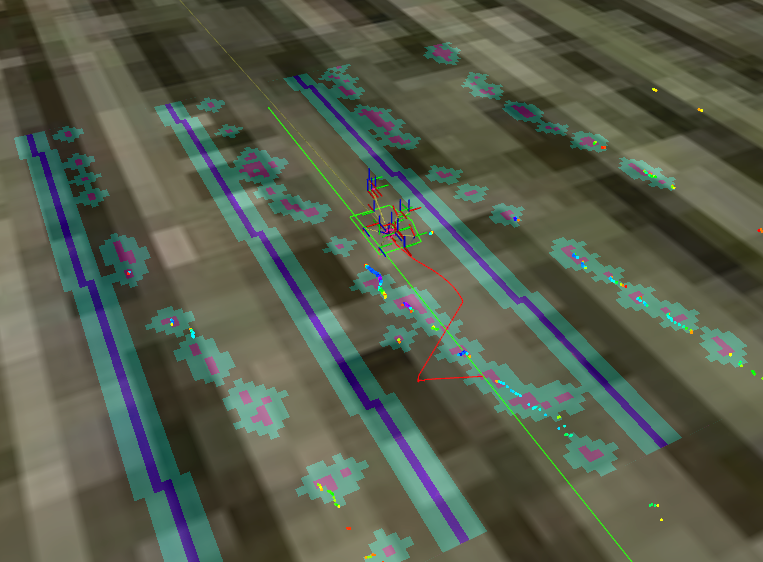
\includegraphics[width=0.8\textwidth]{Images/experimental_data/navigation2_gimped.png}
	\caption{\textit{Visualization through Rviz of the Husky performing autonomous navigation, with the local costmap overlaid to the satellite images of Garriguella vineyard. You can see the global (green line) and local (red line) navigation plans, the} tf \textit{tree of the robot and the Husky footprint used by Move Base for the interaction with the costmap.}}
	\label{fig:result_navigation}
\end{figure}


\section{Manipulation}

As expected, the execution of arm movements through \textit{MoveIt!} framework, when correctly embedded in the unmanned ground vehicle system, gave no surprises in \textit{on-the-field} experiments. In Figure \ref{fig:deplMoveitEndEffect}, you can see the 3D position of the end effector during a grasping and deployment operation, completely executed through \textit{MoveIt!} except, of course, for the core movement of the grasping, the movement 3$\rightarrow$4 in the Figure. The evolution of the $z$ coordinates of the end effector during segment 3$\rightarrow$4 is shown in Figure \ref{fig:graspingZ}.

On the other hand, manipulation sub-operations that relied on computer vision techniques were expected to have problems due to the unpredictable time varying light conditions in outdoor context. A large amount of tests showed two different outcome to \textit{on-the-field} validation:
\begin{itemize}
	\item computer vision tasks based on tracking of ArUco markers (dispenser grasping from the feeder, dispenser application on the nail) turned out to be robust even in presence of the aforementioned light conditions. This is mainly due to the robustness of OpenCV library algorithms in the detection of the markers.
	\item computer vision tasks based on the detection of the red wings of the dispensers (check for dispenser availability in the feeder, grasping and deployment validation) were significantly influenced by the light changes, and they were weaker in the hours about noon, when the sun was on the vertical.
\end{itemize}

In Figure \ref{fig:deploymentNailResult} and \ref{fig:graspingLowResult}, quantitative analysis of visual servo driven movements are provided, through the evolution in time of both the 8 tracked features ($(x,y)$ coordinates for each of the marker corners) and the module of the overall error of the corners with respect to their desired positions. Figure \ref{fig:deploymentNailResult} data comes from the deployment of a dispenser on a nail, while data of Figure \ref{fig:graspingLowResult} comes from the grasping of a dispenser from the feeder. In the graphs related to the feature tracking, the desired value for each of the feature is represented with an horizontal line; notice that, at the end of the execution, each of the features is almost equal to the its target value.


\begin{figure}
	\centering
	\subfloat[]{%
		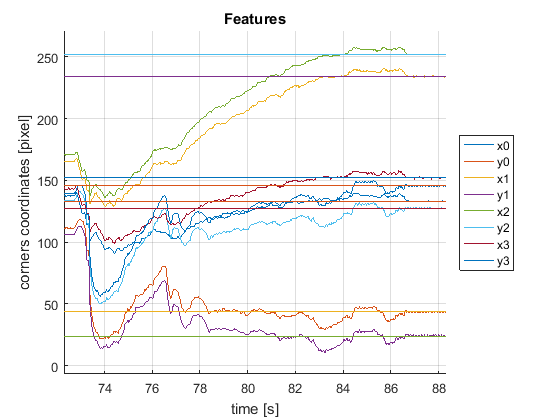
\includegraphics[width=0.65\textwidth]{Images/experimental_data/deployment_nail_features.png}
		\label{fig:deploymentNailFeatures}}
	\subfloat[]{%
		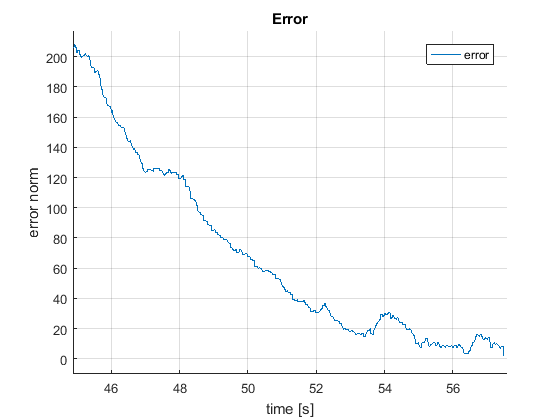
\includegraphics[width=0.65\textwidth]{Images/experimental_data/deployment_nail_error.png}
		\label{fig:deploymentNailError}}
	\caption{\textit{Evolution in time of the image coordinates of the corners of the tracked marker (see Figure \ref{fig:deploymentNailFeatures}) during visual servoing driven deployment of a dispenser on a nail. In Figure \ref{fig:deploymentNailError}, the evolution in time of the module of the error on the tracked features.}}
	\label{fig:deploymentNailResult}
\end{figure}

\begin{figure}
	\centering
	\subfloat[]{%
		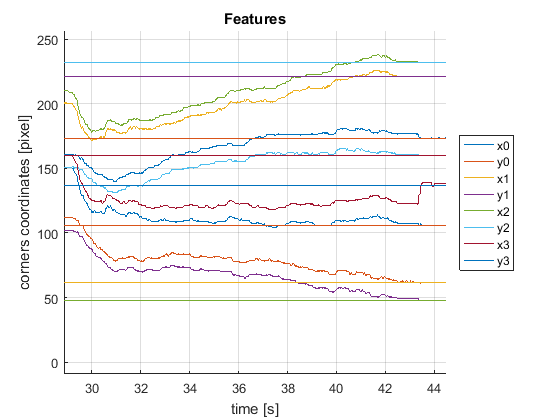
\includegraphics[width=0.65\textwidth]{Images/experimental_data/grasping_low_features.png}
		\label{fig:graspingFeatures}}
	\subfloat[]{%
		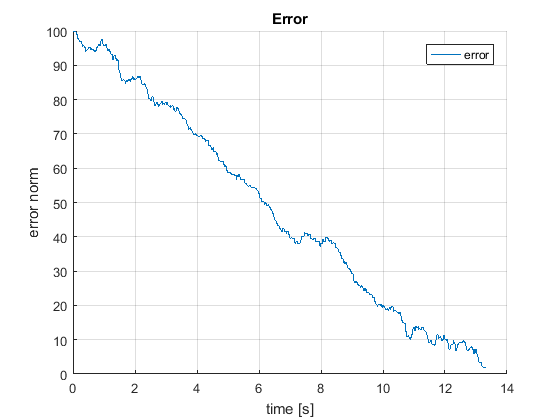
\includegraphics[width=0.65\textwidth]{Images/experimental_data/grasping_low_error.png}
		\label{fig:graspingError}}
	\caption{\textit{Evolution in time of the image coordinates of the corners of the tracked marker (Figure \ref{fig:graspingFeatures}) during visual servoing driven grasping of the dispenser from the feeder. In Figure \ref{fig:graspingError}, the evolution in time of the module of the error on the tracked features,}}
	\label{fig:graspingLowResult}
\end{figure}



\begin{figure}
	\centering
	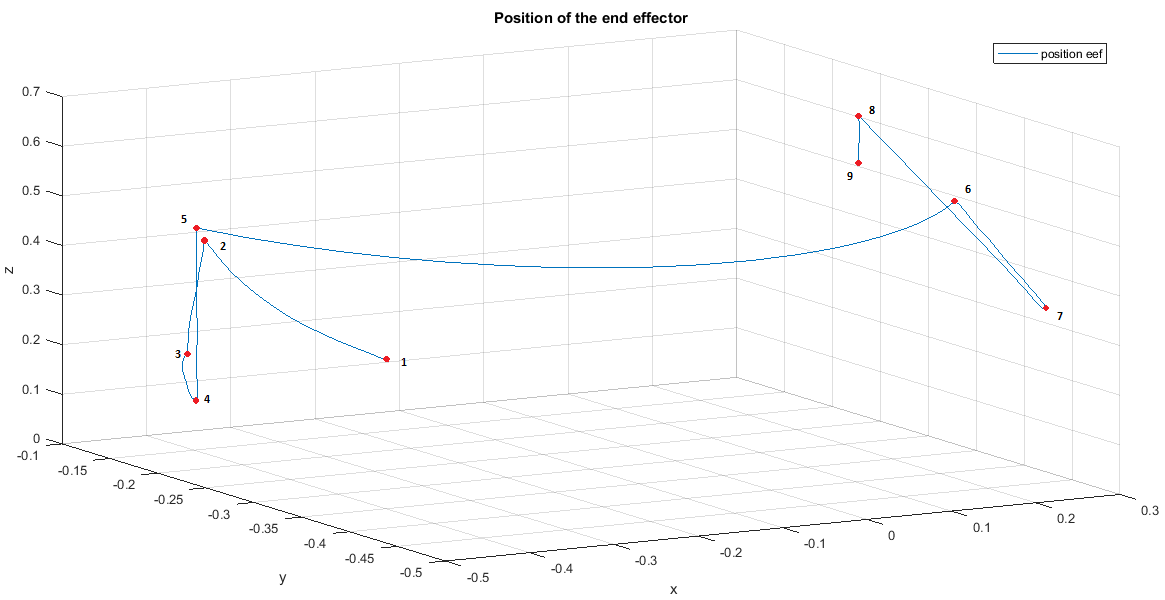
\includegraphics[width=0.9\textwidth]{Images/experimental_data/depl_moveit_endeffector.png}
	\caption{\textit{Evolution of the 3D $(x,y,z)$ position of the end effector of the Jaco$^2$ during dispenser deployment using MoveIt!}}
	\label{fig:deplMoveitEndEffect}
\end{figure}

\begin{figure}
	\centering
	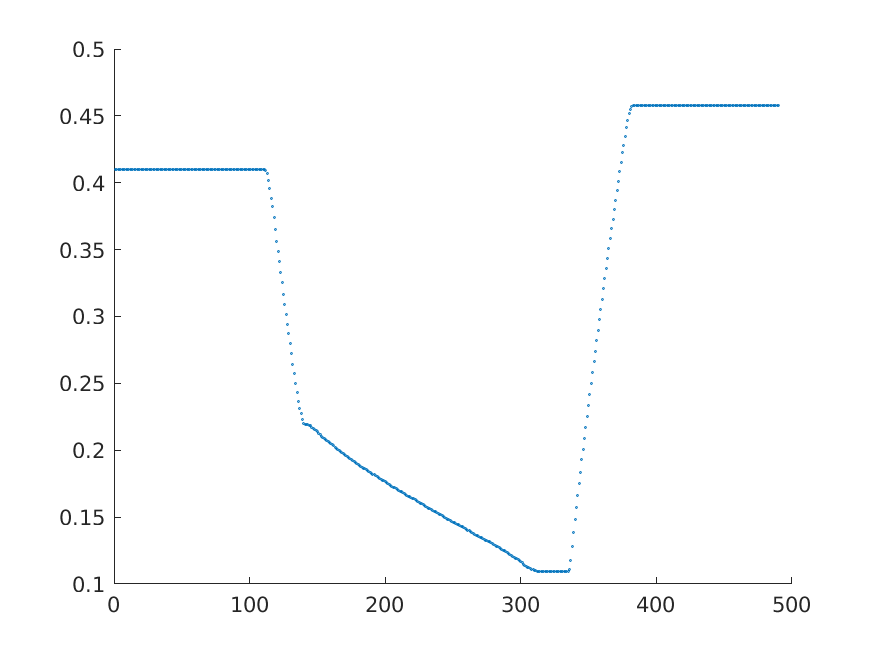
\includegraphics[width=0.7\textwidth]{Images/experimental_data/grasping_z.png}
	\caption{\textit{Evolution of the $z$ coordinate of the end effector, during grasping operation; visual servo driven movement is the central one in the graph.}}
	\label{fig:graspingZ}
\end{figure}






